\section{Mining Movie Heterogeneous Network}
\par (prupose\dots) A movie heterogeneous information network (\emph{MHIN}) is a domain information network with multiple types of entities and relations. We construct our \emph{MHIN} with multiple objects such as movies (M), directors (D), users (U), Actors (A), Types (T) and box-offices (B). Figure \ref{fig:mhin} shows typical \emph{MHIN} schema defined by us. Links exist between users and movies denoting score and score-by relations, between movies and actors(directors) denoting star(direct) and star-by(direct-by) relations, between movies and types denoting label and (labeled) relations, between movies and box-offices denoting gain and gain by relations. Also, we can add other attributes into the movie heterogeneous network (e.g years (Y), producers (P)). Meta-path is a connect relation between two types of objects in \emph{MHIN}. Denote network schema for our \emph{MHIN} is $\mathcal{S}=(\mathcal{A}, \mathcal{R})$, where $\mathcal{A}$ represent object types and $\mathcal{R}$ indicate different types of relationships. A meta-path $\mathcal{P}$ is defined in the form of $A_1 \xrightarrow{R_1} A_2\xrightarrow{R_2} \dots\xrightarrow{R_k} A_{k+1}$. Length of $\mathcal{P}$ is defined by number of relations it contains. Semantic composite relations are implied in meta-paths. For example, we can evaluate the similarity of movies or actors by length-2 meta-path MDM (movie-director-movie), MAM (movie-actor-movie) or AMA (actor-movie-actor), AMTMA(actor-movie-type-movie-actor).

\begin{figure}[!htbp]
\centering
\subfloat[Structure of movie heterogeneous network]{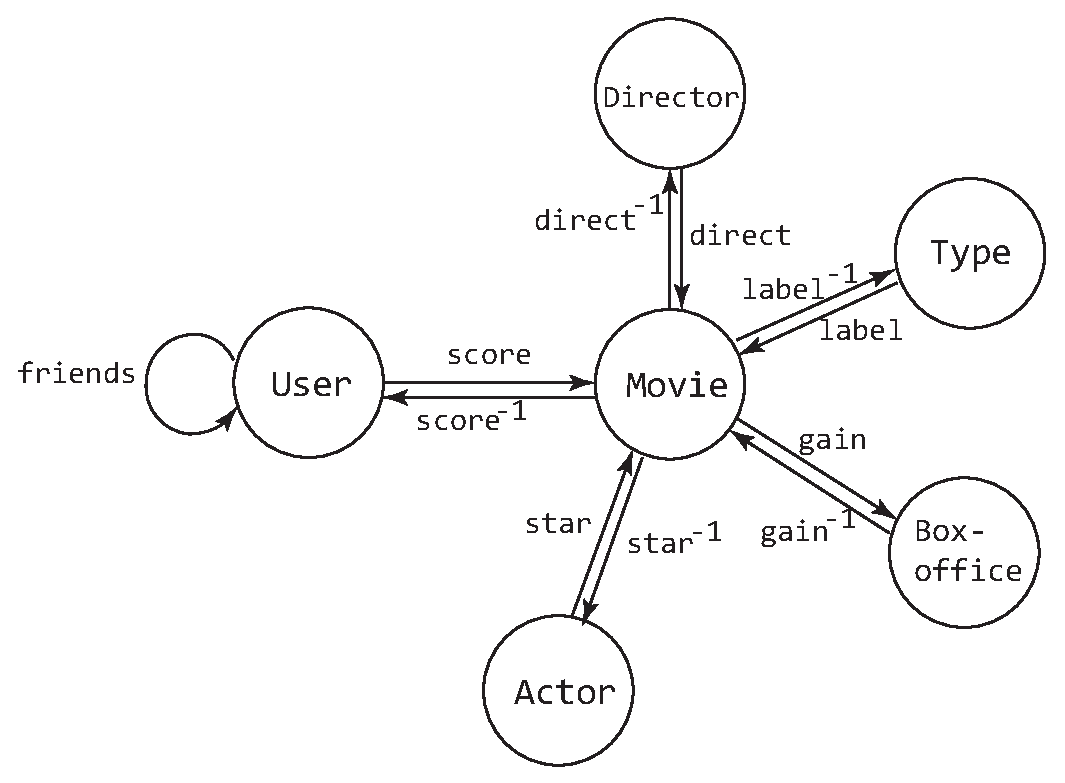
\includegraphics[width=0.8\columnwidth]{mhin.eps}}
\caption{Social network schema of MHIN.}
\label{fig:mhin}
\end{figure}

\subsection{Rank Based Cluster For Actors}
In this section, we introduce a way to make distinguish between A-list and B-list actors. We prefer applying cluster based classifier on actors popularity recognition. Strong available mutually reinforcing relations between cluster and rank are helpful to deal with different levels of actors. We defined recursion formula by following empirical rules.
\newtheorem{rules}[theorem]{rule}
\begin{rules} high rank actors star more high rank movies\end{rules}
\begin{rules} high rank movies attract more high rank actors\end{rules}
\begin{rules} actors get high rank with high rank co-starers\end{rules}

Suppose we want $K$ clusters of actors. According the star relationship between actors and movies, we define matrix $M_{MA}(i, j)=c_{ij}$ representing actor $j$'s contribution of movie $i$ (see Section 3.1) and similarly, $M_{AA}(i, j)= m_{ij}$ stands for number of movies that actor $i$ and actor $j$ co-stared. Note that $W_{AM} = W_{MA}^T$, and $i=\{1,2,\dots, m\}, j=\{1,2,\dots, n\}$. According the 3 rules we proposed, we have

\begin{subequations}
\begin{align}
  r_{A}(i) = \alpha \sum_{i=1}^{m}W_{AM}&(j, i)r_M(i) + (1-\alpha)\sum_{j=1}^{n}W_{AA}(i, j)r_A(j)\\
  r_{A}(j) &\leftarrow \frac{r_{A}(j)}{\sum_{j'=1}^{n}r_{A}(j')}\\
  r_{M}(i) &= \sum_{j=1}^{n}W_{MA}(i, j)r_A(j)\\
  r_{M}(i) &\leftarrow \frac{r_{M}(i)}{\sum_{i'=1}^{m}r_{M}(i')}
\end{align}
\end{subequations}

Note that $\alpha \in [0,1]$ is a believe factor of weighed component of rule 3,  $r_{A}(j)$ and $r_{M}(i)$ are normalized rank score vector. We finally get $r_A$ which should be primary eigenvector of $\alpha W_{AM}W_{MA} + (1-\alpha) W_{AA}$. Further, we capture posterior probability $\pi_{i,k}$ that $a_i$ from cluster $k$, Once an actor acts a movie, he is more likely to star high ranked film and for movie, its success are more likely contributed by high rank actor. Thus we have K dimensional vector $s_{a_i} = \{\pi_{i,1}, \pi_{i,2}, \dots, \pi_{i,K}\}$ where $\pi_{i,k}$ denotes $a_i$'s coefficient for component $k$.

The cluster center and the distance between each actor and each cluster can be defined as
\begin{subequations}
\begin{align}
  S_{A_k} &= \frac{\sum_{a \in A}s(a)}{|A_k|} \\
  Distance(a, A_k) &= 1-\cos(s_{a_i}, S_{A_k})
\end{align}
\end{subequations}

\begin{algorithm}[htb]
\renewcommand{\algorithmicrequire}{\textbf{Input:}}
\renewcommand\algorithmicensure {\textbf{Output:} }
\caption{RankClus for Actors}

\begin{algorithmic}[1]

\REQUIRE ~~\\
Our movie information network $MHIN=(M, A; W)$\\
Cluster Number $K$\\

\ENSURE ~~\\
$K$ clusters of actors $A_i$ and rank of actor in each cluster \\
\STATE iter = 0;
\STATE Init partitions for A, get $PA^{iter}=\{A_i^{iter}\}_1^K$;
\STATE Repeat following until $PA^{iter}-PA^{iter-1}<\epsilon$ or iterations reach limitation
\STATE \quad For all cluster calculate $r_A$ followed by rank function
\STATE \quad Evaluate $\Theta$ for mixture model and get component efficient estimations $s_{a_i}$ for each actor $a_i$
\STATE \quad Update centers $S_{A_k}^{iter}$ of each cluster $A_k$
\STATE \quad Reassign each actor $a_i$ according distance between $a_i$ and each cluster center $A_k^{iter}$
\end{algorithmic}
\end{algorithm}


\subsection{Alternative Actors}
In this section, we discuss method choosing alternative actors for casting agents. The basic idea is measure similarity between actors. Since movie information network has been built, we then introduce meta path-based similarity framework for alternative actors.

\begin{table}[!htb]
  \centering
  \begin{tabular}{c|c|c}
  \hline
  Type & Path instance & Meta-path \\
  \hline
  I(\emph{AMA})& Andy-$M_1$-Sara & Actor-Movie-Actor  \\
  \hline
  II(\emph{AMTMA}) & \tabincell{c}{John-$M_2$-Comedy-$M_3$-Sara\\Ben-$M_4$-War-$M_3$-Sara\\Drew-$M_5$-Dracula-$M_2$-John} & \tabincell{c}{Actor-Movie-\\Type-Movie-Actor} \\
  \hline
  III(\emph{AMDMA}) & \tabincell{c}{Diana-$M_6$-Spielberg-$M_1$-Andy\\John-$M_2$-Luc Besson-$M_5$-Drew\\Sara-$M_3$-Tom Tykwer-$M_5$-Drew} & \tabincell{c}{Actor-Movie-\\Director-Movie-Actor}\\
  \hline
  \end{tabular}
  \caption{Different Types of meta-path in MHIN}\label{tab:metapath}
\end{table}


